\section{Prevalence of datasets containing symbolic features }\label{sec:review}
% \begin{itemize}
%     \item Maxime \ok ? \no ?
%     \item Thierry \ok ? \no ?
%     \item Victor \ok ? \no ?
% \end{itemize}


\begin{table}[h!]% h asks to places the floating element [h]ere.
  \caption{symbolic data}
  \label{tab:catData}
  \begin{footnotesize}
  \begin{center}
  \begin{tabular}{llc}
    \toprule
    Color & Store & Sales \\
    \midrule
    blue  & Paris    & 14 \\
    pink  & Rome     & 12 \\
    pink  & Rome     & 13 \\
    \dots & \dots    & \dots \\
    blue  & Berlin     & 17 \\
    pink  & Paris     & 8  \\
  \bottomrule
\end{tabular}
\end{center}
\end{footnotesize}
\end{table}


\begin{Vocabulary*}
We call \textit{symbolic feature} a component of the input vector. On Table \ref{tab:catData}, \textit{color} and \textit{stores} are symbolic features. We call \textit{symbol} one of the possible value for the feature. On Table \ref{tab:catData} \textit{pink} and \textit{blue} are symbols and forms the \textit{color} alphabet.
\end{Vocabulary*}


While symbolic features are almost absent in computer vision, audio \dots they are critical in many important domains. It is particularly true in health as shown by \cite{PublicHealth}, \cite{HIV} and \cite{SPECT}; diseases or treatments are keen to be symbolic. In supply chain also, symbolic features are ubiquitus. One can find a great supply chain example in \cite{SCPricing} with symbolic features such as $\{$ product group ; vendor ; country ; \dots $\}$. 

It stresses the need to correctly handle symbolic data in modern Machine Learning models, even the gradient-based ones. According to us, every new method machine learning method should not only perform on MNIST from \cite{MNIST} and ImageNet from \cite{IMAGENET} but also on symbolic datasets.

\newline

We highlight two different issues on symbolic features in open datasets. First very few datasets contains symbolic features while those who do are very small. Second many of the symbolic data.We only consider \textit{input} features, we do not mind if the \textit{target} feature is symbolic or numeric.

\\


%% \subsection{No symbolic feature}
Most common datasets used in recent Machine Learning do not contains symbolic data and are thus not encoded. Symbolic features are almost absent from open source datasets. To support this assertion, we investigate three main sources of open datasets in Table \ref{tab:review} and report those tagged as \textit{symbolic} or \textit{categorical}. Datasets reported as symbolic presents at least one symbolic feature in input.




\begin{table}[h!]
  \caption{symbolic features reviews}
  \label{tab:catFeatReview}
  \begin{footnotesize}
  \begin{center}
  \begin{tabular}{lccc}
    \toprule
    Source & datasets & symbolic  & \%  \\
    \midrule
    Kaggle\footnote{\url{https://www.kaggle.com/}{https://www.kaggle.com/}} & $50k$  & $528$ & $1\%$   \\
    UCI \cite{UCI}                                                          & $515$  & $93$  & $18\%$  \\
    data.world \footnote{\url{https://data.world/datasets/open-data}}                         & $130k$ & $91$  & $0.07\%$       
\end{tabular}
\end{center}
\end{footnotesize}
\label{tab:review}
\end{table}


Even though those tags can be incomplete, it indicates how symbolic features are underrepresented in open source datasets. Moreover among the 11 datasets presented by \cite{RevisitingDeepForTabular} that addresses \textit{tabular datasets} (that are the most inclined to contain some!), only \cite{incomeDataset} presents symbolic features.


%% \subsection{Very few data}
While looking for datasets containing symbolic features, we mainly find very small datasets. On the $37$ symbolic datasets available on UCI Machine Learning Repository \cite{UCI}, $22$ have less than $1000$ instances as depicted in Figure \ref{fig:size}. Modern deep learning architectures work with numerical feature and need a lot of data to be trained. Which leads to few datasets with symbolic feature as a vicious circle.

\begin{figure}[h!]
  \centering
  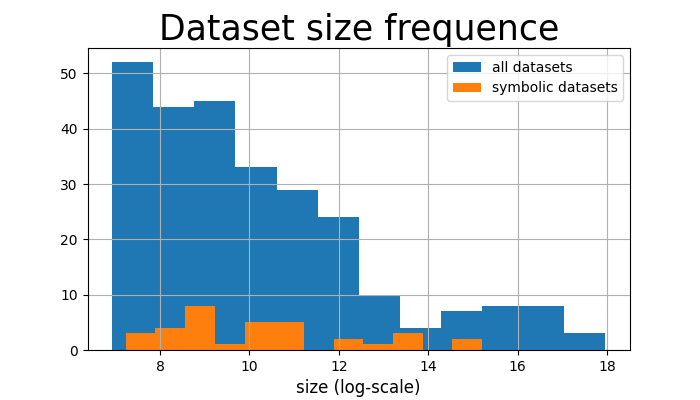
\includegraphics[width=0.5\linewidth]{figures/dataset-size-frequence.png}
  \caption{Size analysis of datasets presented by \cite{UCI}  with more than 1000 instances.
  }
  \label{fig:size}
\end{figure}

%% \subsection{Not really symbolic}
Many encountered \textit{symbolic features} have a latent order as addressed by\cite{OCD}. For example the dataset introduced by  \cite{CarDataset}, which contains cars characteristics, presents a \textit{symbolic feature} ``the size of luggage boot``. This feature often can be ordinaly encoded into a numerical feature following the latent order:

\begin{equation*}
    small \leq med \leq big
\end{equation*}

This remark also applies on binary features, such as boolean ones, that are sometimes recorded as symbolic as in the work of \cite{SPECT} but can directly be treated as numerical. Classical methods on numerical data can applied to those ones.
%%\vfill
These remarks stress the need and the difficulty to correctly handle symbolic features in all machine learning methods, even the gradient-based ones.

